\begin{thm}{024}{\hosi 6}{Jr. 算オリ Final}
 ひし形ABCDに$\mr{AE}=\mr{CF}$となる点を図のように取ります。図のようにア~エの4つの図形に分けると、アはウより155 cm${}^2$小さく、イはエより31 cm${}^2$小さいです。アの面積は何cm${}^2$ですか。
 \begin{center}
  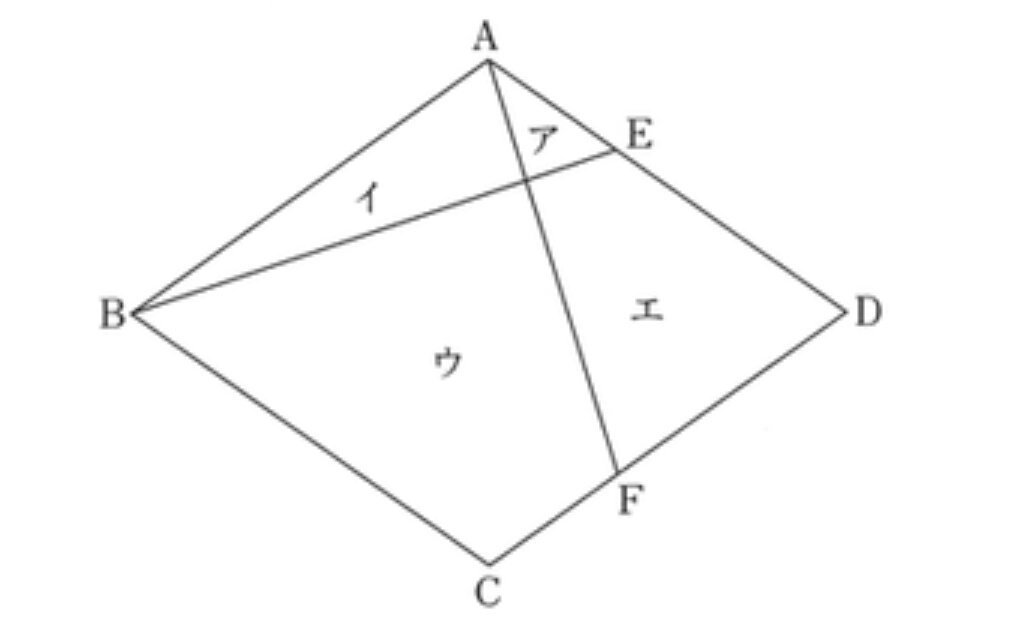
\includegraphics[bb=0 0 1013 637,width=0.7\linewidth]{../problems/Q_024/Q_024.jpg}
 \end{center}
\end{thm}

線分$\mr{CE}$と$\mr{BF}$を引き、点$\mr{G}$, $\mr{H}$を図のように定める。線分$\mr{AF}$と$\mr{BC}$をそれぞれ延長し、交点を$\mr{I}$とする。
\begin{figure}[H]
 \centering
 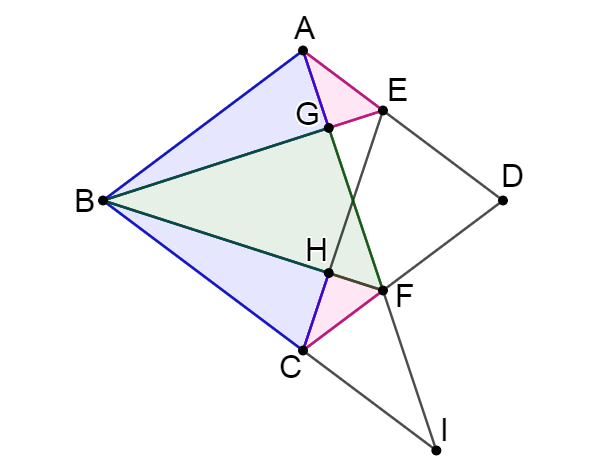
\includegraphics[width=0.6\linewidth]{../problems/Q_024/A_024.png}
\end{figure}
このとき、$\triangle\mr{AEG}=\triangle\mr{CFH}=\text{ア}$、$\triangle\mr{BAG}=\triangle\mr{BCH}=\text{イ}$、$\triangle\mr{CFH}+\triangle\mr{BCH}+\triangle\mr{BFG}=\text{ウ}$である。一方、$\text{ア}+155=\text{ウ}$だから、
\[ \triangle\mr{BCH}+\triangle\mr{BFG}=\triangle\mr{BAG}+\triangle\mr{BFG}=\triangle\mr{ABF}=155 \]
となる。ここで$\triangle\mr{ABF}$はひし形$\mr{ABCD}$の半分の面積を持つから、
\[ \triangle\mr{BCF}+\triangle\mr{ADF}=\text{イ}+\text{ア}+\text{ア}+\text{エ}= 2\times\text{ア}+2\times\text{イ}+31=155 \]
となって、$\text{ア}+\text{イ}=\triangle\mr{BCF}=62$, $\triangle\mr{ADF}=93$を得る。したがって、$\mr{CF}:\mr{DF}=2:3$。ひし形の辺の長さを$a$とすれば、
\begin{align*}
 \mr{EG}:\mr{BG}&=\mr{AE}:\mr{IB} \quad(\because \triangle\mr{AEG}\sim\triangle\mr{IBG}) \\
 &=\frac{2}{5}a:\frac{5}{3}a \quad (\because \mr{AE}=\mr{CF} \,,\,\, \triangle\mr{ADF}\sim\triangle\mr{ICF}) \\
 &=6:25
\end{align*}
したがって、アとイはあわせて62を$6:25$にわけるから、$\text{ア}=12~\mr{cm}^2$と求まった。